\documentclass[../../main.tex]{subfiles}

\begin{figure}[h]
    \centering
    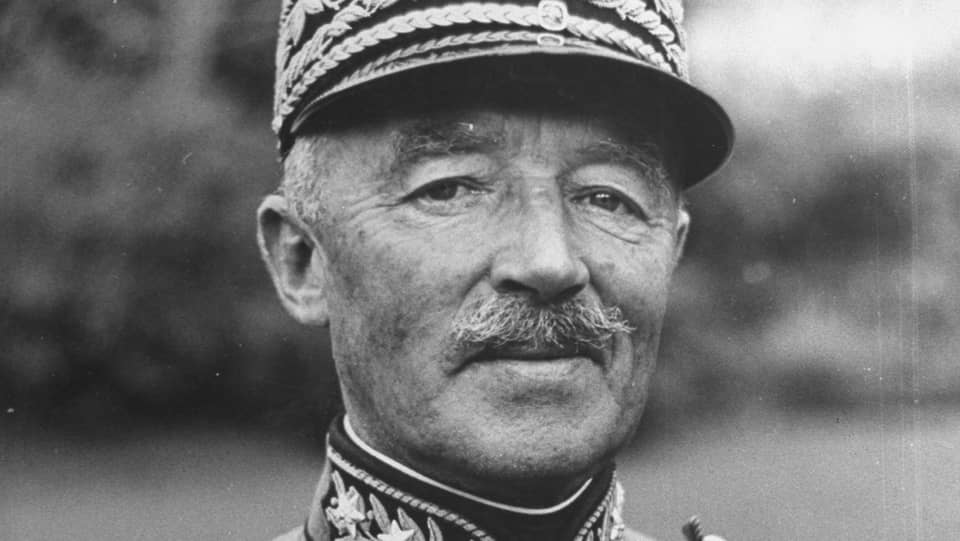
\includegraphics[width=\textwidth,height=7cm,keepaspectratio]{images/guisan.jpg}
    \caption[{Henri Guisan (o.J.). Wikipedia. (27. Juni 2019). \newline URL: https://upload.wikimedia.org/wikipedia/commons/2/2b/Guisan\char`_Visp\char`_1942\char`_D2.8916.jpg [Stand 24.08.2019] }] {Henri Guisan}                                                                                                                                                                                                                                                                                                                 
\end{figure}

Henri Guisan wurde am 21. Oktober 1874 in Mézières geboren. Er war der Sohn von Charles-Ernest Guisan, einem Landarzt, und Louise-Jeanne Bérangier. Seine Mutter starb bereits zehn Monate nach seiner Geburt.

Nach dem Gymnasium lebte Henri Guisan für sechs Monate in Deutschland, um sein Deutsch zu verbessern. Danach begann er ein Medizinstudium, später wechselte er aber zu einem landwirtschaftlichen Studium.

Vor seiner Zeit als General hatte Henri Guisan bereits mehrere Dienstgrade in der Armee inne. Er begann 1894 als Leutnant und wurde 1932 Oberstkorpskommandant. Während des Ersten Weltkrieges war Guisan mehrmals an der deutschen Ostfront, um verschiedene Kriegstaktiken zu erlernen. Als sich die feindliche Stimmung in Europa verstärkte und der Krieg in unangenehme Nähe vorrückte, wurde Henri Guisan am 30. August 1939 zum General und somit zum Oberbefehlshaber der Schweizer Armee gewählt. Die Schweiz hat zu Kriegszeiten einen General, der von der Vereinigten Bundesversammlung, also National- und Ständerat, gewählt wird.

Im Gegensatz zu Ulrich Wille, dem General aus dem Ersten Weltkrieg, war General Guisan äusserst beliebt, da er auch zu den einfachen Soldaten Kontakt pflegte. Mit verschiedensten Ansprachen stärkte er den Wehrwillen der Schweizer Soldaten und der Bevölkerung.

Für Aufsehen sorgte General Guisan mit dem sogenannten «Rütli-Rapport». Am 25. Juli 1940 fuhr er mit allen Armeeangehörigen ab Stufe Major mit dem Dampfschiff Stadt Luzern zur Rütliwiese. Zu diesem Zeitpunkt war die Schweiz von Feinden umzingelt. General Guisan teilte auf der Rütliwiese seinen Entscheid mit, die Armee in das Reduit zurückzuziehen, obwohl er zuvor kein Freund der sogenannten Reduit-Strategie war.

Nach Ende des Zweiten Weltkrieges trat Henri Guisan am 20. August 1945 aus seinem Amt als General ab.

Henri Guisan starb im Alter von 86 Jahren am 7. April 1960. Zu der Trauerfeier am 12. April kamen rund 300'000 Menschen, darunter der gesamte Bundesrat und viele ehemalige Bundesräte.